
\begin{frame}
  \frametitle{Сходимост}
  \vskip-1.5ex
  \begin{equation*}
   \Delta Q_N = |Q_N - I| \propto \frac{\sqrt{\mathrm{Var}(h)}} {\sqrt{N}} \pause = \frac{\sigma_N} {\sqrt{N}}
  \end{equation*}
  \pause
  \vskip-6.5ex
  \begin{figure}[t]
  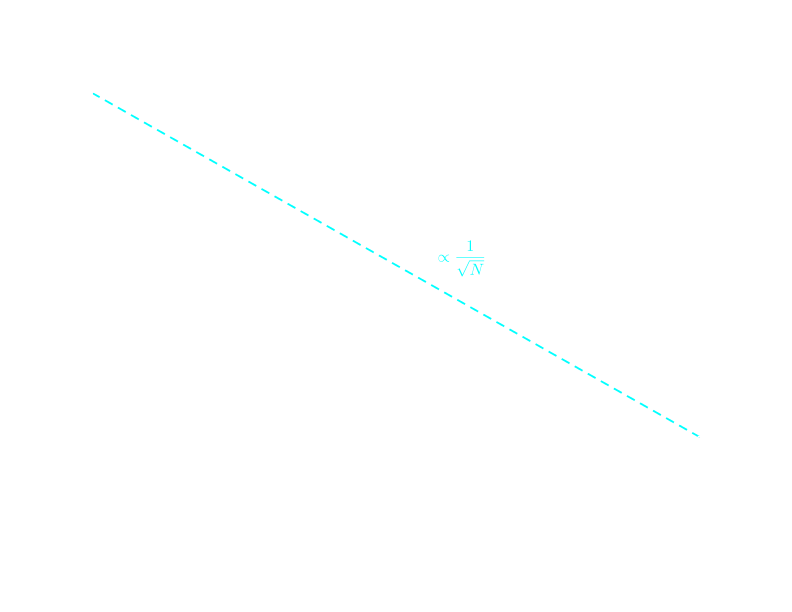
\includegraphics[width=0.7\textwidth]{mc_error2.png}
  \end{figure}
\end{frame}

\begin{frame}
  \frametitle{Сходимост}
  \makebox[\textwidth]{
  \animategraphics[width=\textwidth,autoplay]{2}{animated/montecarlo-}{0}{12}
  }
  \begin{table}
  \begin{tabular}{l | c }
              & Сходимост    \\
  \hline \hline
  Монте Карло & $\mathcal{O}(N^{-1/2})$  \\
      &     \\
  \end{tabular}
  \end{table}
\end{frame}

\begin{frame}
  \frametitle{Сходимост}
  \makebox[\textwidth]{
  \animategraphics[width=\textwidth,autoplay]{2}{animated/trapez-}{0}{12}
  }
  \begin{table}
  \begin{tabular}{l | c }
              & Сходимост    \\
  \hline \hline
  Монте Карло & $\mathcal{O}(N^{-1/2})$  \\
  \pause
  Трапеците   & $\mathcal{O}(N^{-2/s})$    \\
  \end{tabular}
  \end{table}
\end{frame}
%\begin{frame}
%  \frametitle{Сходимост}
%  \begin{table}
%  \begin{tabular}{l | c | c }
%            &   1-D  &  S-D   \\
%\hline \hline
%Монте Карло & 
%$\mathcal{O}(N^{-1/2})\propto \sqrt{\mathrm{Var}(h)}$   & $\mathcal{O}(N^{-1/2})$ \\ \pause 
%Трапеците   & $\mathcal{O}(N^{-2}) \propto d^2h(x)$  & $\mathcal{O}(N^{-2/s})$ \\ \pause
%Симпсон     & $\mathcal{O}(N^{-4})$      & $\mathcal{O}(N^{-4/s})$ \\ 
%Квази МК    & $\mathcal{O}(log(n) n^{-1})$ & $\mathcal{O}(log(n)^s n^{-1})$ \\
%\end{tabular}
%\caption{Сходимост на методи за числено интегриране}
%\end{table}
%\end{frame}

\begin{frame}
%  \frametitle{Сходимост}
  \vskip-0.5ex
  \begin{figure}[t]
    \includegraphics[height=8.0cm]{convergence.png}
  \end{figure}
\end{frame}
